\subsection{Dawn and dusk sides}

Aside from short time and local variations, we also are interested in images showing simultaneously the two sides
of Titan. At low phase angle, the viewing geometry allows us to retrieve the haze extinction with both the
illuminated and the dark side of Titan simultaneously  (Fig.~\ref{fig:dawn_dusk}).
In this case, we can compare the dawn and dusk limbs for
specific latitudes. Although Titan's day is about 16 terrestrial
days, the time spent by the haze on the night side or dayside is much shorter.
First, the atmosphere is superrotating and at altitude around 400 or 500 km the zonal wind is comparable to or
larger than the rotation speed at the ground \citep{Flasar2005, Achterberg2011, Lebonnois2012, Lellouch2019}.
This makes the actual diurnal cycle for the high altitude hazes shorter than 16 days by a factor of 2 or more.
Secondly, at high altitude, sunlight penetrating beyond the geometric terminator further shortens the time spent in darkness.
Thus, effects on the haze should be produced by processes with timescales
comparable with a terrestrial day.

\begin{figure}[!ht]
\plotone{Fig/Dawn_dusk}
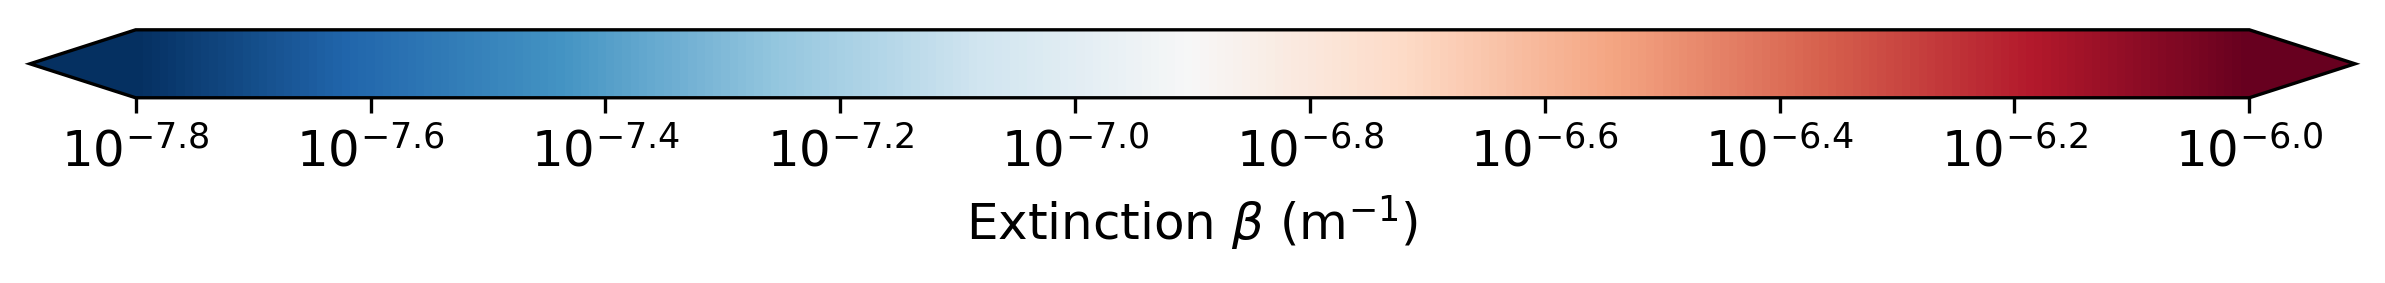
\includegraphics[width=.5\textwidth]{Fig/Extinction_colorbar}
\caption{The left and right panels show maps of the haze extinction for the dawn and dusk side of
Titan for 4 different images taken during the mission when the viewing geometry allows us to observe both dawn and dusk
limbs. The date and the seasonal solar longitude are provided for each image.}
\label{fig:dawn_dusk}
\end{figure}

Figure~\ref{fig:dawn_dusk}a presents the haze extinction at the dawn and dusk sides as observed
in June of 2005 (Fig.~\ref{fig:dhl_2004_2008}c). The detached haze differs significantly between the two sides.
At the equator, we observe on the dawn side a double detached layer of 40 km thickness whereas it appears
as a thin layer of 10 km thickness on the dusk side. The haze extinction at the peak differs significantly,
from 7$\times 10^{-8}$ to 2.5$\times 10^{-8}$ m$^{-1}$, respectively. The depletion below the haze layer
is also less pronounced on the dawn side compared to the dusk side. Although this observation was taken
during the period of stability for the detached haze, we observed a significant asymmetry between
the dawn and dusk side. This asymmetry is also observed in all the images taken at the same moment which were
analyzed in section 4.1.

Two years later, another low phase angle image was recorded (Fig.~\ref{fig:dawn_dusk}b).
This time, the detached haze layer is much more symmetrical between the two sides. The peaks of haze extinction
are at the same altitude with comparable values. However, small differences can be noticed: there is a
small secondary layer above the detached haze layer at the dusk side between \ang{50}S and \ang{20}N, and may even extend
northward. In the northern hemisphere, the extinction appears slightly larger at dawn that at dusk, and the
vertical extent of the detached haze is also a bit larger. However, the overall morphologies are very similar.

At the equinox, the detached haze layer already started its drop in altitude (Fig.~\ref{fig:dawn_dusk}c).
There are significant differences between the two sides, in both hemispheres, while at the equator the two
profiles are almost identical. The haze layer is not exactly symmetrical in the southern hemisphere. The detached
haze itself is at the same altitude, but the depletion zone is at higher altitude at the dawn side, and the main
haze layer is thinner in the dusk side. In the northern hemisphere, the haze layer is more complex, and the
asymmetry is even more marked with a detached haze at different altitudes and with a different extinction. The
detached and main haze layers at the dawn side appear optically thicker than the layers at the dusk side.
This is consistent with the two previous cases.

After the equinox, fewer images were taken at low phase angle. Among them, we do not notice any
significant differences between the dawn and dusk sides. After the reappearance of the detached haze layer in
2016, we found only one image with the relevant geometry to see both sides of Titan illuminated at the same time
(Fig.~\ref{fig:dawn_dusk}d). In this case, we are close to the solstice and the sub-solar latitude is almost
at its maximal extent and does not allow us to probe the southern high latitudes near the terminator.
The main haze appears very symmetrical on both sides and almost identical
above \ang{45}N. The depletion can be followed continuously all around the North Pole. At latitudes lower than
\ang{45}N, the values of the haze extinction are similar but the altitudes of the extinction peak differ by
25 km. We also observe partial secondary detached layers in each side, but not at the same latitudes.

The haze extinction profile and the altitude of the detached haze layer can differ significantly between the dawn
and dusk sides. In general we notice a higher extinction in the dawn side than on the dusk side. This effect
could be due to a diurnal cycle.